\documentclass[10pt]{beamer}

\usetheme[progressbar=frametitle]{metropolis}
\usepackage{appendixnumberbeamer}

% \usepackage{enumitem}

\usepackage{booktabs}
\usepackage[scale=2]{ccicons}

\usepackage{pgfplots}
\usepgfplotslibrary{dateplot}

\usepackage{xspace}
\newcommand{\themename}{\textbf{\textsc{metropolis}}\xspace}


\setbeamercolor{alerted text}{fg=teal}
\setbeamercolor{emph}{fg=teal}
\renewcommand<>{\emph}[1]{%
  {\usebeamercolor[fg]{emph}\only#2{\itshape}#1}%
}

\title{An Invitation to \newline Mathematical Quantum Physics}
\subtitle{Lancaster University Postgraduate Forum}
% \date{\today}
\date{}
\author{Luke Mader}
\institute{Lancaster University}

\usepackage[export]{adjustbox}
\usepackage{amsmath,
            amssymb,
            gensymb,
            mathtools
            }

\usepackage{textcomp} % i forget this package's purpose

% \usepackage{pgfplots}
% \pgfplotsset{width=10cm}
\linespread{1.8}


\usepackage{amsthm}

\newcommand{\set}[1]{\left\{#1\right\}}
\newcommand{\N}{\mathbb{N}}
\newcommand{\R}{\mathbb{R}}
\newcommand{\Z}{\mathbb{Z}}
\newcommand{\Q}{\mathbb{Q}}
\newcommand{\C}{\mathbb{C}}
\newcommand{\M}{\mathrm{M}}
\newcommand{\F}{\mathbb{F}}
\newcommand{\HS}{\mathcal{H}}

\newcommand{\eps}{\varepsilon}
\newcommand{\id}{\text{id}}
\newcommand{\dist}[1]{\text{dist}\left(#1\right)}
\newcommand{\ip}[1]{\left\langle #1\right\rangle}
\newcommand{\conjugate}[1]{\mkern 1.5mu\overline{\mkern-1.5mu#1\mkern-1.5mu}\mkern 1.5mu} 
\newcommand{\dom}[1]{\mathrm{Dom}\left(#1\right)}


\DeclarePairedDelimiter\abs{\lvert}{\rvert}%
\DeclarePairedDelimiter\norm{\lVert}{\rVert}%

% Swap the definition of \abs* and \norm*, so that \abs
% and \norm resizes the size of the brackets, and the
% starred version does not.
\makeatletter
\let\oldabs\abs
\def\abs{\@ifstar{\oldabs}{\oldabs*}}
%
\let\oldnorm\norm
\def\norm{\@ifstar{\oldnorm}{\oldnorm*}}
\makeatother


\newcommand{\op}[1]{\norm{#1}_\text{op}}



% bra-ket notation
% uses package mathtools
\DeclarePairedDelimiter\bra{\langle}{\rvert}
\DeclarePairedDelimiter\ket{\lvert}{\rangle}
\DeclarePairedDelimiterX\braket[2]{\langle}{\rangle}{#1 \vert #2}
\DeclarePairedDelimiterX\ketbra[2]{\delimsize\vert}{\delimsize\vert}{#1 \rangle\langle #2}





\newcommand*{\rvec}[1]{\left( #1\right)}
\newcommand*{\tr}[1]{\operatorname{tr}\left(#1\right)}
\newcommand*{\range}[1]{\operatorname{range}\left(#1\right)}
\renewcommand*{\ker}[1]{\operatorname{ker}\left(#1\right)}


\begin{document}

\metroset{block=fill}
\maketitle

\begin{frame}{A quantum particle living in \(\R\)}
    Suppose that we have a quantum particle contained inside of \(\R\).

    \bigskip

    This particle has things we can observe: e.g. \emph{position}, \emph{momentum}, and \emph{energy}. Such things are called \emph{observables}.
\end{frame}

\begin{frame}{Wave-particle duality}
  Quantum objects can be observed to have both wave-like and particle-like properties. This is known as \emph{wave-particle duality}.

  % \only<2>{\begin{figure}[H]
  %   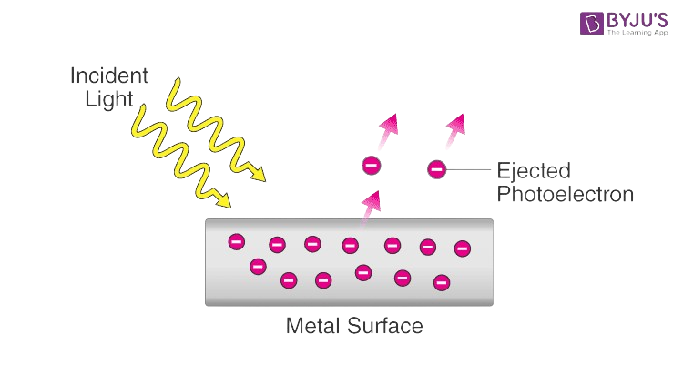
\includegraphics[scale=0.4]{photo_electric_effect.png}
  % \end{figure}
  % }
  % \only<3>{\begin{figure}[H]
  %   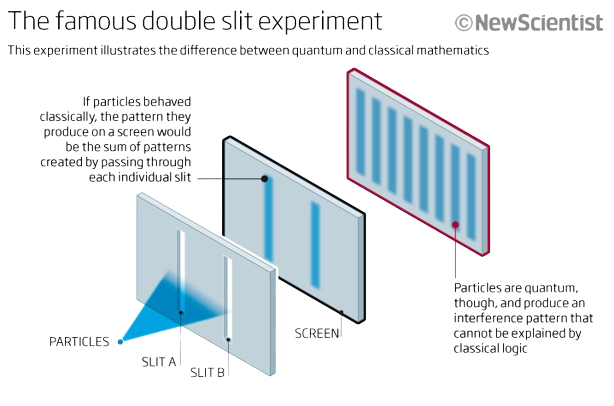
\includegraphics[scale=0.4]{double_slit.png}
  % \end{figure}
  % }
  \begin{figure}[H]
      \includegraphics<1>[scale=0.4]{c_photoelectric-effect.png}
      \includegraphics<2>[scale=0.4]{c_double_slit.jpg}
  \end{figure}

\end{frame}

\begin{frame}{Probabilistic behaviour of quantum objects}
  In the double-slit experiment, electrons that are `identical' \emph{do not hit the screen at the same point}.

  \medskip

  \pause This suggests that we \emph{cannot predict the outcome} of a quantum experiment; we can only predict \emph{the probabilities of an outcome} of a quantum experiment.
\end{frame}

\begin{frame}{The wavefunction}
  The \emph{wavefunction} combines the \emph{probabilistic nature} and \emph{wave-particle duality} of a quantum object. \newline It is a \emph{mathematical} encoding of what we know about the particle. 

  \pause For a particle moving in \(\R\) dependent on time \(t \in \R\), the wavefunction is some map \(\psi \colon \R \times \R \to \C\).
  \begin{itemize}
    \pause \item \(\mathbb{P}\bigl( \text{The position of the particle is in \(E \subset \R\)} \bigr) = \int_{E} \abs{\psi(x)}^2 \,\mathrm{d}x\).
    \pause \item The \emph{time-evolution} of the particle is \emph{wave-like}: \begin{equation*}
        \frac{\partial \psi}{\partial t} = \frac{1}{i\hbar}H\psi.
    \end{equation*} This is the famous \emph{Schr{\"o}dinger equation}.
  \end{itemize}
\end{frame}

\begin{frame}{An underlying space for wavefunctions}
 As \(\mathbb{P}\bigl( \text{The position of the particle is in \(E \subset \R\)} \bigr) = \int_{E} \abs{\psi(x)}^2 \,\mathrm{d}x\), clearly 
 \begin{equation*}
  \mathbb{P}\bigl( \text{The position of the particle is in \(\R\)} \bigr) = 1 = \int_{\R} \abs{\psi(x)}^2 \,\mathrm{d}x.
 \end{equation*}
 \pause Therefore, it makes sense to associate the wavefunctions with the space \(\mathrm{L}^2(\R)\), where 
 \begin{equation*}
    f \in \mathrm{L}^2(\R) \longleftrightarrow \int_{\R} \abs{f(x)}^2 \,\mathrm{d}x < \infty.
 \end{equation*}
 
 This is not technically the definition of \(\mathrm{L}^2(\R)\), but it is good enough as a working definiton. To make this more precise, we need measure theory.  
\end{frame}

\begin{frame}{Properties of \(\mathrm{L}^2(\R)\)}
  \begin{itemize}
    \item \(\mathrm{L}^2(\R)\) is an \emph{infinite-dimensional vector space}.
    \pause\item \(\ip{\phi, \psi} \coloneqq \int_{\R} \conjugate{\phi(x)} \psi(x) \,\mathrm{d}x\) is an inner product on \(\mathrm{L}^2(\R)\), and \begin{equation*}
      \norm{\psi} \coloneqq \left( \int_{\R} \abs{\psi(x)}^2 \,\mathrm{d}x\right)^{\frac{1}{2}} = \sqrt{\ip{\psi, \psi}}
    \end{equation*} 
    defines a norm on \(\mathrm{L}^2(\R)\) where \emph{every Cauchy sequence converges}. 
    \pause\item \(\mathrm{L}^2(\R)\) has a non-trivial \emph{dense subset}. 
  \end{itemize}
\end{frame}

\begin{frame}{The position operator}
  As \(\ip{\phi, \psi} = \int_{\R} \conjugate{\phi(x)} \psi(x) \,\mathrm{d}x\), we can express the expectation of the position as 
  \begin{equation*}
    \mathbb{E}(x) \coloneqq \int_{\R} x \abs{\psi(x)}^2 \,\mathrm{d}x = \ip{\psi(x), x\psi(x)}.
  \end{equation*}
  \pause We therefore have a natural operator describing the position of our particle: 
  \begin{equation*}
    X \colon \mathrm{Dom}(X) \to \mathrm{L}^2(\R),
    \qquad 
    X(\psi) \coloneqq x\psi(x).
  \end{equation*}  
  \pause An issue: \(\mathrm{Dom}(X) \neq \mathrm{L}^2(\R)\), as \begin{equation*}
    \frac{1}{x} \chi_{[1, \infty)}(x) \in \mathrm{L}^2(\R) \quad\text{but}\quad \chi_{[1, \infty)}(x) \not\in \mathrm{L}^2(\R)
  \end{equation*}
\end{frame}

\begin{frame}{What have we seen so far?}
  \begin{itemize}
    \item Quantum particles behave both as \emph{waves} and \emph{particles}, and have a \emph{probabilistic nature}. We describe this through \emph{wavefunctions, which encode everything we know about the particle}.
    \pause\item A natural space for wavefunctions is \(\mathrm{L}^2(\R)\). 
    \pause\item For a wavefunction \(\psi\), \(\abs{\psi}^2\) can be interpreted as a \emph{probability density function}.
    \pause\item Through the inner product of \(\mathrm{L}^2(\R)\), we can get an operator describing the position of a particle. This operator \emph{cannot be defined on the whole space}.
  \end{itemize}
\end{frame}

\begin{frame}{Hilbert spaces}
  A (complex, infinite-dimensional) \emph{Hilbert space \(\HS\)} is a (complex, infinite-dimensional) vector space such that:
  \begin{itemize}
    \item For a given inner product \(\ip{\cdot, \cdot}\), \(\norm{\cdot} \coloneqq \sqrt{\ip{\cdot, \cdot}}\) is a norm.
    \item Every Cauchy sequence converges with respect to this norm (\(\HS\) is \emph{complete}).
    \item If \(\HS\) has a dense countable subset, then it is \emph{separable}. 
    % \newline \(S\) is dense in \(\HS\) if \begin{equation*}
    %   \conjugate{S}
    %   \coloneqq 
    %   S \cup \set{\lim_{n \to \infty} x_n \in \HS \,\colon \left(x_n\right)_{n = 1}^{\infty} \text{is in \(S\) and converges}} 
    %   = \HS.
    % \end{equation*}
  \end{itemize}
\end{frame} 

\begin{frame}{Operators on Hilbert Spaces}
  A linear map \(T \colon \HS \to \HS\) is a \emph{bounded operator} if there exists some \(M > 0\) such that for all \(x \in \HS\), \begin{equation*}
    \norm{Tx} \leq M\norm{x}.
  \end{equation*}

  \pause For a subspace \(\dom{T} \subset \HS\), an \emph{(unbounded) operator} is any linear map \(T \colon \dom{T} \to \HS\).

  An (unbounded) operator is \emph{densely-defined} if \(\dom{T}\) is dense in \(\HS\).
\end{frame}

\begin{frame}{Adjoints of bounded operators}
  For a bounded operator \(T\colon \HS \to \HS\), there exists an \emph{adjoint} operator \(T^* \colon \HS \to \HS\) defined by \begin{equation*}
    \ip{x, Ty} = \ip{T^*x, y}
  \end{equation*}  
  for any \(x, y \in \HS\). Furthermore, \emph{the adjoint operator is unique}.
\end{frame}

\begin{frame}{Existence of adjoints of bounded operators}
  \begin{theorem}[Riesz-Fr{\'e}chet theorem]
    For a Hilbert space \(\HS\) and a continuous linear map \(\psi \, \colon \HS \to \C\), there is a unique \(z \in \HS \) such that for all \(y \in \HS\), \begin{equation*}
      \psi(y) = \ip{z, y}.
    \end{equation*}
  \end{theorem}
  Fix \(x \in \HS\). Then, \(\psi \colon \HS \to \C \), \(\psi(y) = \ip{x, Ty}\) is a continuous linear map. By the Riesz-Fr{\'e}chet theorem, there exists a unique \(z \in \HS\) such that \begin{equation*}
    \ip{z, y} = \ip{x, Ty}.
  \end{equation*}
  Define \(T^*\) by \(T^* x = z\) to get a linear bounded operator.
\end{frame}

\begin{frame}{What about adjoints of unbounded operators?}
  Let \(T \colon \dom{T} \to \HS\) be a \emph{densely-defined} operator. Define \[
    \dom{T^*} 
    \coloneqq
    \set{x \in \HS \colon y \mapsto \ip{x, Ty} \,\text{where \(y \in \dom{T}\) is a continuous map}}. 
  \]
  \vspace{-1cm}
  \begin{itemize}
    \item \(\dom{T^*}\) is a subspace.
    \item As \(\dom{T}\) is dense, there exists a unique extension of \(x \mapsto \ip{x, Ty}\) to the entirety of \(\HS\) for every \(y \in \HS \). \newline By the Riesz-Fr{\'e}chet theorem, there then exists a unique vector \(z \in \HS\) such that \begin{equation*}
      \ip{z, y} = \ip{x, Ty}
    \end{equation*}
    for all \(y \in \dom{T}\) and \(x \in \dom{T^*}\). Define \(T^*\) by \(T^*x = z\).
  \end{itemize}
\end{frame}

\begin{frame}{Consequences of this construction}
  \begin{itemize}
    \item We need the denseness of \(\dom{T}\) or else the uniqueness of the adjoint fails. Therefore, \emph{only densely-defined operators have adjoints}.
    \pause \item In general, \(\dom{T} \neq \dom{T^*}\). Nightmarishly, 
    \begin{enumerate}
      \pause \item \(\dom{T^*}\) may not be dense, so \((T^*)^*\) \emph{may not exist}.
      \pause\item There exist operators such that \(\dom{T} \cap \dom{T^*} = \set{0}\).
      \pause\item For two densely-defined operators \(T\) and \(S\) on \(\HS\), as \[\dom{T + S} = \dom{T} \cap \dom{S},\] \emph{\(T + S\) may have no adjoint}.
    \end{enumerate}
  \end{itemize}
\end{frame}

\begin{frame}{Symmetric and self-adjoint operators}
  An operator \(T \colon \dom{T} \to \HS\) is \emph{symmetric} if for all \(x, y \in \dom{T}\), \begin{equation*}
    \ip{x, Ty} = \ip{Tx, y}.
  \end{equation*}
  If \(T\) is densely-defined, symmetric, and if \(\dom{T} = \dom{T^*}\), then \(T\) is \emph{self-adjoint}.

  \pause\begin{theorem}
    A densely-defined operator \(T \colon \dom{T} \to \HS\) is symmetric if and only if \(T^*\) is an extension of \(T\).
  \end{theorem}
\end{frame}

% \begin{frame}{Graphs and closures of operators}
%   The \emph{graph} of an operator \(T\colon \dom{T} \to \HS \) is defined by \[
%     \mathrm{G}(T)
%     \coloneqq
%     \set{
%       (x, Tx) \in \HS \oplus \HS 
%       \colon 
%       x \in \dom{T}
%     }.
%   \] 
%   \vspace{-1cm}
%   \begin{itemize}
%     \pause\item Graphs uniquely determine operators.
%     \pause\item The \emph{closure of an operator} \(T\) is the operator \(\conjugate{T}\) with the graph \(\conjugate{\mathrm{G}(T)}\). 
%   \end{itemize}
% \end{frame} 

\begin{frame}{Essentially self-adjoint operators}
  An operator \(T \colon \dom{T} \to \HS\) is \emph{essentially self-adjoint} if:
  \begin{itemize}
    \item \(T\) is symmetric: \(\ip{x, Ty} = \ip{Tx, y}\) for all \(x,y \in \dom{T}\).
    \item The operator \(\conjugate{T}\) whose \emph{graph} is given by the \emph{closure of the graph of \(T\)}, \begin{equation*}
    \mathrm{G}(\conjugate{T})
    =
    \conjugate{\mathrm{G}(T)}
    =
    \conjugate{
      \set{
        (x, Tx) \in \HS \oplus \HS 
        \colon 
        x \in \dom{T}
      }
    },
    \end{equation*} is self-adjoint.
  \end{itemize}

  \bigskip
  
  \pause If \(T\) is essentially self-adjoint, then \(\conjugate{T}\) is \emph{the unique self-adjoint extension of \(T\)}.
\end{frame}

\begin{frame}{Our friend the position operator}
  Recall the position operator \(X \colon \dom{X} \to \mathrm{L}^2(\R)\) given by \[X(\psi) = x\psi(x).\]
  \vspace{-1cm}
  \begin{itemize}
    \pause \item \(X\) is self-adjoint on \[\dom{X} = \set{\psi \in \mathrm{L}^2(\R) \colon x\psi(x) \in \mathrm{L}^2(\R)}.\]
    \vspace{-.7cm}
    \pause \item \(X\) is not self-adjoint but is essentially self-adjoint on \[ 
      \mathcal{S}(\R) 
      \coloneqq 
      \set{
        \psi \in \mathrm{C}^\infty (\R)
        \colon 
        \forall \alpha, \beta\in \N, \,
        \sup_{x \in \R} \abs{x^\alpha \frac{\mathrm{d^\beta}\psi(x)}{\mathrm{d}x^\beta}} < \infty
      }.
    \]
  \end{itemize}
\end{frame}

\begin{frame}{What have we seen so far?}
  \begin{itemize}
    \item \emph{Bounded operators always have an adjoint} and are always either \emph{self-adjoint or not self-adjoint}. 
    \pause \item For unbounded operators, \emph{only densely-defined operators have adjoints}. There are \emph{different families of unbounded operators between self-adjoint and not self-adjoint}.
    \pause\item \emph{Changing the domain} of an unbounded operator \emph{can change key properties} of the operator.
  \end{itemize}
\end{frame}

\begin{frame}{The axioms of quantum mechanics}
  To formalise what we originally saw in quantum physics, we introduce the following `axioms':
  \begin{enumerate}
    \item The \emph{possibile states} of a quantum system are \emph{associated with vectors} in a complex and separable Hilbert space that have \emph{norm 1}.
    \pause\item \emph{Observables} in our quantum system are associated with \emph{self-adjoint linear operators}.
    \pause\item If an observation \(a\) has the corresponding operator \(A\) and if our quantum system is in the state \(\psi \in \dom{A}\), then the \emph{expected value for the measurement of \(a\)} is \begin{equation*}
      \mathbb{E}_{\psi}(A) = \ip{\psi,A\psi}.
    \end{equation*}
  \end{enumerate}
\end{frame}

\begin{frame}{The 1D quantum harmonic oscillator}
  The \emph{Hamiltonian} operator describes the \emph{energy} of a quantum system.
  
  \medskip 

  \pause For the quantum harmonic oscillator, it is the operator \(H \colon \dom{H} \to \mathrm{L}^2(\R)\) given by \begin{equation*}
    H = \frac{1}{2m} \bigl(P^2 + (m\omega X^2)\bigr),
  \end{equation*}
  where:
  \begin{itemize}
    \item \(P\psi = -i\hbar \frac{\mathrm{d}\psi}{\mathrm{d}x}\) is the \emph{momentum operator}
    \item \(X\psi = x\psi(x)\) is the \emph{position operator}
  \end{itemize}
\end{frame}

\begin{frame}{The mathematical problem}
  A natural domain for our Hamiltonian is the \emph{Schwartz space}, \begin{equation*}
    \dom{H} 
    = \mathcal{S}(\R)
    = \set{
      \psi \in \mathrm{C}^\infty (\R)
      \colon 
      \forall \alpha, \beta \in \N, \,
      \sup_{x \in \R} \abs{x^\alpha \frac{\mathrm{d^\beta}\psi(x)}{\mathrm{d}x^\beta}} < \infty
    }.
  \end{equation*}
  \pause Our goals: \begin{itemize}
    \item Find the \emph{eigenvalues} (if they exist) of our Hamiltonian on \(\mathcal{S}(\R)\): these are \emph{the energy levels of the quantum harmonic oscillator}.
    \pause \item Confirm that the Hamiltonian is either \emph{essentially self-adjoint} or \emph{self-adjoint} on \(\mathcal{S}(\R)\) so that we \emph{satisfy our axioms}.
  \end{itemize}
\end{frame}

\begin{frame}{Simplifying our problem}
  We introduce the following two operators:
  \begin{align*}
    &\text{Lowering Operator:} &a \colon \mathcal{S}(\R) &\to \mathrm{L}^2(\R), &a &= \frac{1}{\sqrt{2\hbar m \omega}} \Big( m\omega X + iP \Big)\\
    &\text{Raising Operator:} &a^* \colon \mathcal{S}(\R) &\to \mathrm{L}^2(\R), &a^* &= \frac{1}{\sqrt{2\hbar m \omega}} \Big( m\omega X - iP \Big)
  \end{align*}
  \vspace{-1cm}
  \begin{itemize}
    \pause \item \(a^*\) is the adjoint of \(a\) on \(\mathcal{S}(\R)\).
    \pause \item \(a^*a\) is symmetric on \(\mathcal{S}(\R)\).
    \pause \item \(H = \hbar \omega \left(  a^*a + \frac{1}{2}I \right)\) on \(\mathcal{S}(\R)\).
    \pause \item \(\lambda \mapsto \hbar \omega \left( \lambda + \frac{1}{2} \right)\) takes us from the eigenvalues of \(a^*a\) to all of the eigenvalues of \(H\) on \(\mathcal{S}(\R)\).
  \end{itemize}
\end{frame}

\begin{frame}{Eigenvalue results}
  Suppose \((\lambda, \psi)\) is an eigenvalue-eigenvector pair for \(a^*a\) when defined on \(\mathcal{S}(\R)\). Then,
  \begin{itemize}
    \item \(a^*a (a \psi) = (\lambda - 1)a\psi\).
    \item \(a^*a (a^* \psi) = (\lambda + 1) a^* \psi\).
  \end{itemize}
  Therefore, \begin{itemize}
    \item \(a\psi = 0\) or \((\lambda - 1, a\psi)\) is an eigenvalue-eigenvector pair for \(a^*a\).
    \item \(a^*\psi = 0\) or \((\lambda + 1, a^*\psi)\) is an eigenvalue-eigenvector pair for \(a^*a\).
  \end{itemize}
  Important consequence: \emph{if we have an eigenvalue-eigenvector pair for \(a^*a\), we can repeatedly apply \(a\) to the eigenvector to get an eigenvalue of 0}.
\end{frame}

\begin{frame}{Eigenvalue results}
  Suppose that \(a^*a\) has eigenvectors when defined on \(\mathcal{S}(\R)\).
  \begin{itemize}
    \pause\item \emph{Every eigenvalue} of \(a^*a\) is \emph{non-negative}.
    \pause\item There is an eigenvector \(\psi_0\) such that \[
        a\psi_0 = a^*a \psi_0 = 0.
    \]
  \end{itemize}
  \pause As \(a^*a\) has no negative eigenvalues, \(\psi_0\) is the \emph{eigenvector with the lowest possible eigenvalue}. We call this the \emph{ground state for \(a^*a\)}.

  \pause Furthermore, for \(n \geq 0\) define the \emph{excited states} by \(\psi_n \coloneqq (a^*)^n \psi_0\).
  \begin{enumerate}
    \item Any distinct pair \((\psi_n, \psi_m)\) are orthogonal.
    \item \(a^* \psi_n = \psi_{n + 1}\) and \(a \psi_n = n \psi_{n - 1}\), so \emph{\(a^*a \psi_n = n\psi_n\)}.
  \end{enumerate}
\end{frame}

\begin{frame}{The eigenvalues}
  The ground state of \(a^*a\) when defined on \(\mathcal{S}(\R)\) is \begin{equation*}
    \psi_0 (x) = \left(
      \frac{m \omega}{\pi \hbar}
    \right)^{\frac{1}{4}}
    \exp\left(
      -\frac{m\omega}{2\hbar} x^2
    \right).
  \end{equation*}
  \pause The excited states are given by \begin{equation*}
    \psi_n (x) = H_n \left(x\sqrt{\frac{m\omega}{\hbar}}\right) \psi_0 (x),
  \end{equation*}
  where \(H_n\) is the physicist's Hermite polynomial \begin{equation*}
    H_n (y)
    =
    \begin{cases*}
      1 & \text{if \(n = 1\)}.\\
      \frac{1}{\sqrt{2}} \left(2x H_{n - 1} (y) - \frac{\mathrm{d}}{\mathrm{d}x} H_{n - 1} (y)\right) & \text{if \(n \geq 2\)}.
    \end{cases*}
  \end{equation*}
\end{frame}

\begin{frame}{\(a^*a\) and the Hamiltonian are essentially self-adjoint}
  \(a^*a\) is essentially self-adjoint on \(\mathcal{S}(\R)\):
  \begin{itemize}
    \pause \item \(a^*a\) is symmetric on \(\mathcal{S}(\R)\).
    \item The eigenvectors \(\psi_n\) of \(a^*a\) form an orthogonal basis of \(\mathrm{L}^2(\R)\).
  \end{itemize}
  \pause \(H = \hbar \omega \left(  a^*a + \frac{1}{2}I \right)\) is essentially self-adjoint on \(\mathcal{S}(\R)\):
  \begin{itemize}
    \pause \item As \(a^*a\) is symmetric on \(\mathcal{S}(\R)\), \(H\) is as well.
    \item The eigenvectors for \(H\) are the same as for \(a^*a\) on \(\mathcal{S}(\R)\).
  \end{itemize}
  \pause The energy levels of the Hamiltonian on \(\mathcal{S}(\R)\) are given by
  \begin{equation*}
    E_n = \hbar \omega \left(  n + \frac{1}{2}\right) \qquad \text{for \(n \in \N\)}.
  \end{equation*}
\end{frame}

\begin{frame}[plain]
  \begin{center}
    {\Huge Thanks for listening!}
  \end{center}
\end{frame}

\begin{frame}[allowframebreaks]{References}

  \bibliography{references}
  \bibliographystyle{abbrv}

\end{frame}
\end{document}
